% !TEX encoding = UTF-8
% !TEX TS-program = pdflatex
% !TEX root = ../Tesi.tex

%************************************************

%************************************************


L'argomentazione rappresenta un approccio al ragionamento nei casi in cui si dispone di conoscenza inconsistente, e può essere considerata come un metodo per gestire l’incertezza. Infatti, l’idea alla base dell'argomentazione è quella di valutare il motivo per cui un fatto sia considerato vero analizzando gli argomenti e le relazioni che intercorrono tra essi per valutarne la certezza. Tale processo può essere visto come una forma di ragionamento riguardo gli argomenti per determinarne i più accettabili. Sebbene il termine argomentare possa intuitivamente richiamare diversi significati come quello del ragionamento a partire da premesse fino alle conclusioni o l'esprimere la propria opinione in una discussione, un argomento non si lega a particolari strutture ma in senso astratto è qualsiasi cosa che può attaccare o essere attaccata da un altro argomento. Per tale motivo, un Argumentation Framework può essere adeguato a rappresentare diverse situazioni. La possibilità dell'Argumentation Framework di poter rappresentare diverse situazioni ha portato, nel tempo, alla proposta di estensioni che ponessero attenzione su diversi aspetti, come i tipi di relazione che possono sussistere o la quantificazione della forza di una relazione tra due argomenti.

\section{Argumetation Framework}
La definizione iniziale formulata da Dung prevede esclusivamente la presenza di relazioni di attacco tra argomenti e non permette di assegnare un peso a ciascuna relazione per indicare la forza di un attacco \cite{dung1995acceptability}. Successivamente, tali aspetti sono stati considerati in particolari estensioni dell'AF, come quella del Bipolar Argumentation Framework (BAF), che prevede relazioni di attacco e di supporto tra gli argomenti, e quella del Weighted Argumentation Framework (WAF), in cui le relazioni di attacco sono pesate.


\subsection{Argumetation Framework di Dung}
Si riporta di seguito la descrizione formale dell'argumentation framework di Dung \cite{dung1995acceptability}, che costituisce l’argumentation framework più semplice, contenente solamente relazioni di attacco tra argomenti.

\bigskip
\begin{defn} \textbf{Argumentation Framework (AF)}. Un Argumentation Framework (AF) è una coppia ⟨A,R⟩, dove A è un insieme di argomenti, R ⊆ A × A è una relazione binaria. Dati due argomenti a, b ∈ A, se esiste una coppia ⟨a, b⟩ ∈ R significa che a attacca b. Un insieme S ⊆ A attacca b se b è attaccato da un argomento in S. Un insieme S di argomenti attacca un insieme S' di argomenti se esiste un argomento a ∈ S che attacca un argomento b ∈ S'.
\end{defn}

Un argumentation framework $\mathcal{AF = ⟨A,R⟩}$ può essere rappresentato come un grafo orientato $\mathcal{G = ⟨V, E⟩}$, dove l’insieme dei nodi $\mathcal{V}$ corrisponde all'insieme $\mathcal{A}$ e l’insieme degli archi $\mathcal{E}$ corrisponde all'insieme $\mathcal{R}$.

\bigskip
\begin{exmp}
    Sia dato l'$\mathcal{AF = ⟨A, R⟩}$, dove:
    \begin{center}
        $\mathcal{A} = ⟨a, b, c, d, e, f, g, h⟩$
        
        $\mathcal{R} = \{⟨a, b⟩, ⟨b, c⟩, ⟨c, d⟩, ⟨a, e⟩, ⟨e, d⟩, ⟨e, f ⟩, ⟨f, g⟩, ⟨g, e⟩, ⟨f, h⟩, ⟨h, f ⟩\}$
    \end{center}
    
    \begin{figure}
      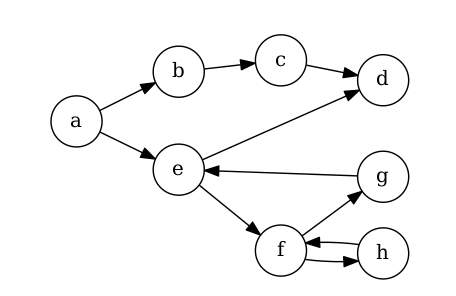
\includegraphics[width=\linewidth]{Immagini/example-graph.png}
      \caption{Rappresentazione del grafo.}
      \label{fig:graph1}
    \end{figure}
    
    \label{exm:af}
\end{exmp}

\bigskip
\begin{defn} \textbf{Difesa} Sia dato un argumentation framework $\mathcal{AF = ⟨A, R⟩}$ Un argomento a $\mathcal{∈ A}$ è difeso da un insieme di argomenti $\mathcal{S ⊆ A} $ e per ogni argomento b  $\mathcal{∈ A}$ vale che se ⟨b, a⟩ $\mathcal{∈ R}$ allora b è attaccato da $\mathcal{S}$.
\end{defn}

Ad esempio, nell'$\mathcal{AF}$ definito nell'esempio \ref{exm:af}, {a} difende c perché b, attaccante di c, è a sua volta attaccato da a.

\bigskip
\begin{defn} \textbf{Conflict-free} Sia dato un argumentation framework AF =
⟨A, R⟩. Un insieme S ⊆ A è conflict-free se e solo se non esistono due argomenti a, b ∈ S tali che ⟨a, b⟩ ∈ R.
\end{defn}  

Ad esempio, nell'$\mathcal{AF}$ definito nell'esempio \ref{exm:af}, \{a, c, g, h\} è conflict-free perché non presenta argomenti in relazione tra di loro.

\bigskip
\begin{defn} \textbf{Stable extension} Sia dato un argumentation framework
$\mathcal{AF = ⟨A, R⟩}$. Un insieme $\mathcal{S ⊆ A}$ conflict-free è una stable extension se e solo se per ogni argomento c $\mathcal{∈ A}$ tale che c $\mathcal{∉ S}$ vale che esiste un argomento b $\mathcal{∈ S}$ tale che ⟨b, c⟩ $\mathcal{∈ R}$.
\end{defn}

Ad esempio, nell'$\mathcal{AF}$ definito nell'esempio \ref{exm:af}, l'insieme delle stable extension è costituito da $\{\{a, c, f \}, \{a, c, g, h\}\}$.

\bigskip
\begin{defn} \textbf{Admissible extension} Sia dato un argumentation framework $\mathcal{AF = ⟨A, R⟩}$. Un insieme $\mathcal{S ⊆ A}$ conflict-free è una admissible extension se e solo se ogni argomento in $\mathcal{S}$ è difeso da $\mathcal{S}$.
\label{adm-ext-dung}
\end{defn}

Ad esempio, nell'$\mathcal{AF}$ definito nell'esempio \ref{exm:af}, l'insieme delle stable extension è costituito da \{∅, \{a\}, \{h\}, \{a, c\}, \{a, f\}, \{a, h\}, \{g, h\}, \{a, c, f \}, \{a, c, h\}, \{a, g, h\},
\{a, c, g, h\}\}.

\bigskip
\begin{defn} \textbf{Preferred extension} Sia dato un argumentation framework $\mathcal{AF = ⟨A, R⟩}$. Un insieme $\mathcal{S ⊆ A}$ è una preferred extension se è una admissible
extension massimale rispetto all'inclusione insiemistica.
\end{defn}

Ad esempio, nell'$\mathcal{AF}$ definito nell'esempio \ref{exm:af}, l'insieme delle preferred extension è costituito da \{\{a, c, f \}, \{a, c, g, h\}\}.

\bigskip
\begin{defn} \textbf{Complete extension} Sia dato un argumentation framework $\mathcal{AF = ⟨A, R⟩}$. Un insieme $\mathcal{S ⊆ A}$ ammissibile è una complete extension se e solo se ogni argomento che è difeso da $\mathcal{S}$ appartiene ad $\mathcal{S}$.
\end{defn}

Ad esempio, nell'$\mathcal{AF}$ definito nell'esempio \ref{exm:af}, l'insieme delle complete extension è costituito da \{\{a, c\}, \{a, c, f \}, \{a, c, g, h\}\}.

\bigskip
\begin{defn} \textbf{Grounded extension} Sia dato un argumentation framework $\mathcal{AF = ⟨A, R⟩}$. Un insieme $\mathcal{S ⊆ A}$ è la grounded extension se è una complete extension minimale rispetto all'inclusione insiemistica.
\end{defn}

Ad esempio, nell'$\mathcal{AF}$ definito nell'esempio \ref{exm:af}, la grounded extension è costituita da \{\{a, c\}\}.

\bigskip
\begin{prp}Ogni stable extension è anche una preferred extension, ma non il contrario. Inoltre, ogni preferred extension è anche una complete extension. Possono esistere più stable, preferred e complete extension, ma la grounded extension è unica.
\end{prp}

Per quanto riguarda i cicli presenti in un argumentation framework, valgono le seguenti proprietà:

\bigskip
\begin{prp}. Se un argumentation framework $\mathcal{AF = ⟨A,R⟩}$ non ha alcun ciclo di lunghezza pari, allora l’unica preferred extension di AF è l’insieme vuoto.
\end{prp}

\bigskip
\begin{prp}. Se un argumentation framework $\mathcal{AF = ⟨A,R⟩}$ non ha alcun ciclo di lunghezza dispari, allora ogni preferred extension di AF è una stable extension.
\end{prp}

\bigskip
\begin{prp}. Se un argumentation framework $\mathcal{AF = ⟨A,R⟩}$ non ha alcun ciclo ed $\mathcal{A = ∅}$, allora $\mathcal{AF}$ ha una singola estensione che è preferred, completa e grounded.
\end{prp}


\subsection{Bipolar Argumetation Framework}
Una estensione dell'argumentation framework di Dung considera il fatto che tra due argomenti non esiste solo una relazione di attacco, ma può esistere anche una relazione di supporto. La distinzione in due tipi di relazioni opposte tra di loro suggerisce la nozione di bipolarismo, ovvero l’esistenza di due tipi di informazioni indipendenti che hanno natura diametralmente opposta e che rappresentano forze di repulsione. Il concetto di bipolarismo è importante quando si devono prendere decisioni in quanto è possibile distinguere informazioni a supporto di una decisione, ed informazioni che la contrastano [1]. Si descrive, di seguito, formalmente il bipolar argumentation framework.

\bigskip
\begin{defn} \textbf{Bipolar Argumentation Framework (BAF)} Un Bipolar Argumentation Framework (BAF) è una tripla $⟨\mathcal{A}, \mathcal{R}_{def}, \mathcal{R}_{sup}⟩$ dove $\mathcal{A}$ è un insieme di argomenti, $\mathcal{R}_{def}$ è una relazione binaria su $\mathcal{A}$ chiamata relazione di attacco e $\mathcal{R}_{sup}$ è una relazione binaria su $\mathcal{A}$ chiamata relazione di supporto. Dati due argomenti $a, b ∈ \mathcal{A}$, $a \mathcal{R}_{def} b ⇔ ⟨a, b⟩ ∈ \mathcal{R}_{def}$ (rispettivamente  $a \mathcal{R}_{sup} b ⇔ ⟨a, b⟩ ∈  \mathcal{R}_{sup}$ ) indica che a attacca b (rispettivamente a supporta b). Un bipolar argumentation framework $BAF = ⟨\mathcal{A}, \mathcal{R}_{def} , \mathcal{R}_{sup} ⟩$ può essere rappresentato come un grafo orientato $\mathcal{G} = ⟨\mathcal{V}, \mathcal{E}⟩$, dove l'insieme dei nodi $\mathcal{V}$ corrisponde all'insieme $\mathcal{A}$ e l'insieme degli archi $\mathcal{E}$ corrisponde all'insieme $\mathcal{R}_{def} ∪ \mathcal{R}_{sup}$. Dati due argomenti $a, b ∈ \mathcal{A}$, $a \mathcal{R}_{def} b$ è rappresentato come $a → b$ e $a \mathcal{R}_{sup} b$ è rappresentato come $a -→ b$.

\end{defn}

\bigskip
\begin{exmp}
    Sia dato il $BAF  = ⟨\mathcal{A}, \mathcal{R}_{def}, \mathcal{R}_{sup}⟩$, dove:
    \begin{center}
        $\mathcal{A} = ⟨a, b, c, d, e, f, g, h⟩$
        
        $\mathcal{R}_{def} = \{⟨c, d⟩, ⟨a, e⟩, ⟨e, f⟩, ⟨f, g⟩, ⟨g, e⟩, ⟨f, h⟩, ⟨h, f⟩\}$
        
        $\mathcal{R}_{sup} = \{⟨a, b⟩, ⟨b, c⟩, ⟨e, d⟩\}$
    \end{center}
    
    \begin{figure}
      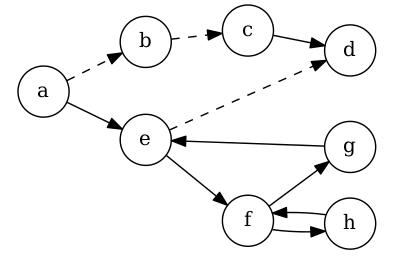
\includegraphics[width=\linewidth]{Immagini/example-baf-graph.png}
      \caption{Rappresentazione del grafo bipolar.}
      \label{fig:baf-graph1}
    \end{figure}
    
    \label{exm:baf}
\end{exmp}

\bigskip
\begin{defn} \textbf{Relazione di Attacco Diretto} 
Sia dato un bipolar argumentation framework $BAF = ⟨\mathcal{A}, \mathcal{R}_{def}, \mathcal{R}_{sup}⟩$ e siano dati due argomenti $a, b ∈ \mathcal{A}$. Se $ a \mathcal{R}_{def} b$ allora si parla di attacco diretto da a verso b.
\label{defn:adbaf}
\end{defn}

Ad esempio, nel $BAF$ definito nell'esempio \ref{exm:baf}, è presente una relazione di attacco diretto da $c$ verso $d$ perchè $⟨c, d⟩ ∈ \mathcal{R}_{def}$.


\bigskip
\begin{defn} \textbf{Relazione di Attacco Indiretto} 
Sia dato un bipolar argumentation framework $BAF = ⟨\mathcal{A}, \mathcal{R}_{def}, \mathcal{R}_{sup}⟩$. Un attacco indiretto verso un argomento $b ∈ \mathcal{A}$ è una sequenza $a_{1}\mathcal{R}_{1}...\mathcal{R}_{n-1}a_{n}$ dove $n \geq 3, a_n = b, \forall i = 2, ..., n-1, \mathcal{R}_i = \mathcal{R}_{sup}$ e $ \mathcal{R}_{1} = \mathcal{R}_{def}$.
\label{defn:aibaf}
\end{defn}

Ad esempio, nel $BAF$ definito nell'esempio \ref{exm:baf}, è presente una relazione di attacco indiretto verso $d$ perchè $⟨a, e⟩ ∈ \mathcal{R}_{def}$ e $⟨e, d⟩ ∈ \mathcal{R}_{sup}$.


\bigskip
\begin{defn} \textbf{Attacco supportato} 
Sia dato un bipolar argumentation framework $BAF = ⟨\mathcal{A}, \mathcal{R}_{def}, \mathcal{R}_{sup}⟩$. Un attacco supportato verso un argomento $b ∈ \mathcal{A}$ è una sequenza $a_{1}\mathcal{R}_{1}...\mathcal{R}_{n-1}a_{n}$ dove $n \geq 3, a_n = b, \forall i = 1, ..., n-2, \mathcal{R}_i = \mathcal{R}_{sup}$ e $ \mathcal{R}_{n-1} = \mathcal{R}_{def}$.
\label{defn:asbaf}
\end{defn}

Ad esempio, nel $BAF$ definito nell'esempio \ref{exm:baf}, è presente un attacco supportato verso $d$ perchè $⟨c, d⟩ ∈ \mathcal{R}_{def}$ e $⟨a, b⟩, ⟨b, c⟩ ∈ \mathcal{R}_{sup}$.


\bigskip
\begin{defn} \textbf{Attacco di insieme} 
Sia dato un bipolar argumentation framework $BAF = ⟨\mathcal{A}, \mathcal{R}_{def}, \mathcal{R}_{sup}⟩$. Un insieme $S \subseteq A$ attacca un argomento $b \in A$ se e solo se esiste un attacco diretto, supportato o indiretto verso $b$ da un elemento di $S$.
\label{defn:adibaf}
\end{defn}

Ad esempio, nel $BAF$ definito nell'esempio \ref{exm:baf}, è presente un attacco di insieme da $S = =\{a, b, c\}$ verso $d$ perchè esiste un attacco supportato dagli elementi $a, b, c \in S$ verso $d$.


\bigskip
\begin{defn} \textbf{Supporto di insieme} 
Sia dato un bipolar argumentation framework $BAF = ⟨\mathcal{A}, \mathcal{R}_{def}, \mathcal{R}_{sup}⟩$. Un insieme $S \subseteq A$ supporta un argomento $b \in A$ se e solo se esiste una sequenza $a_{1}\mathcal{R}_{sup}...\mathcal{R}_{sup}a_{n}$ dove $n \geq 2, a_n = b$ e $a_1 \in S$
\label{defn:sdibaf}
\end{defn}

Ad esempio, nel $BAF$ definito nell'esempio \ref{exm:baf}, è presente un supporto di insieme da $S = =\{a\}$ verso $c$ perchè esiste una sequenza di supporti da $a \in S$ verso $c$.


\bigskip
\begin{defn} \textbf{Difesa} 
Sia dato un bipolar argumentation framework $BAF = ⟨\mathcal{A}, \mathcal{R}_{def}, \mathcal{R}_{sup}⟩$. Un insieme $S \subseteq A$ difende un argomento $a \in A$ se e solo se per ogni argomento $b \in A$, se $b$ attacca $a$ allora $b$ è attaccato da $S$.
\label{defn:dbaf}
\end{defn}

Ad esempio, nel $BAF$ definito nell'esempio \ref{exm:baf}, $e$ difende $g$ perchè $f$, attaccante di $g$, è a sua volta attaccato da $e$.


\bigskip
\begin{defn} \textbf{Conflict-free} 
Sia dato un bipolar argumentation framework $BAF = ⟨\mathcal{A}, \mathcal{R}_{def}, \mathcal{R}_{sup}⟩$. Un insieme $S \subseteq A$ è conflict-free se e solo se non esistono due argomenti $a, b \in S$ tali che sussista un attacco di insieme da $\{a\}$ verso $b$.
\end{defn}

Ad esempio, nel $BAF$ definito nell'esempio \ref{exm:baf}, $\{a, b, c, f\}$ è conflict-free perchè non presenta argomenti coinvolti in attacchi di insieme tra loro.


\bigskip
\begin{defn} \textbf{Safe} 
Sia dato un bipolar argumentation framework $BAF = ⟨\mathcal{A}, \mathcal{R}_{def}, \mathcal{R}_{sup}⟩$. Un insieme $S \subseteq A$ è safe se e solo se non esiste alcun argomento $b \in A$ tale che sussista un attacco di insieme da $\{S\}$ verso $b$ o che ci sia un supporto di insieme da $S$ verso $b$ o che $b \in S$. 
\end{defn}

Ad esempio, nel $BAF$ definito nell'esempio \ref{exm:baf}, $\{b, c\}$ è safe perchè attacca solo $d$, ma non lo supporta; inoltre $d$ non appartiene a tale insieme.


\bigskip
\begin{defn} \textbf{Stable Extension} 
Sia dato un bipolar argumentation framework $BAF = ⟨\mathcal{A}, \mathcal{R}_{def}, \mathcal{R}_{sup}⟩$. Un insieme $S \subseteq A$ conflict-free è una stable extension se e solo se per ogni argomento $a \notin S$ sussiste un attacco di insieme da $S$ verso $a$.
\end{defn}

Ad esempio, nel $BAF$ definito nell'esempio \ref{exm:baf}, l'insieme delle stable extension è costituito da $\{\{a, b, c, f\}, \{a, b, c, g, h\}\}$.


\bigskip
\begin{defn} \textbf{d-admissible extension} 
Sia dato un bipolar argumentation framework $BAF = ⟨\mathcal{A}, \mathcal{R}_{def}, \mathcal{R}_{sup}⟩$. Un insieme $S \subseteq A$ conflict-free è una d-admissible extension se e solo se ogni argomento in $S$ è difeso da $S$. Tale definizione equivale alla definizione \ref{adm-ext-dung} di ammissibilità per l'AF di Dung.
\end{defn}

Ad esempio, nel $BAF$ definito nell'esempio \ref{exm:baf}, l'insieme delle d-admissible extension è costituito da $\{∅, \{a, h\}$, $\{a, b, h\}$, $\{a, c, h\}$, $\{a, b, c, h\}$, $\{a, g, h\}$, $\{a, b, g, h\}$, $\{a, c, g, h\}$, $\{a, b, c, g, h\}$, $\{g, h\}$, $\{c, g, h\}$, $\{b, g, h\}$, $\{b, c, g, h\}$, $\{b, h\}$, $\{b, c, h\}$, $\{c, h\}$, $\{h\}$, $\{a, f\}$, $\{a, b, f \}$, $\{a, c, f \}$, $\{a, b, c, f \}$, $\{a\}$, $\{a, b\}$, $\{a, c\}$, $\{a, b, c\}$, $\{b\}$, $\{b, c\}$, $\{c\}\}$.


\bigskip
\begin{defn} \textbf{s-admissible extension} 
Sia dato un bipolar argumentation framework $BAF = ⟨\mathcal{A}, \mathcal{R}_{def}, \mathcal{R}_{sup}⟩$. Un insieme $S \subseteq A$ safe è una s-admissible extension se e solo se ogni argomento in $S$ è difeso da $S$.
\end{defn}

Ad esempio, nel $BAF$ definito nell'esempio \ref{exm:baf}, l'insieme delle s-admissible extension è costituito da $\{∅, \{a, h\}$, $\{a, b, h\}$, $\{a, c, h\}$, $\{a, b, c, h\}$, $\{a, g, h\}$, $\{a, b, g, h\}$, $\{a, c, g, h\}$, $\{a, b, c, g, h\}$, $\{g, h\}$, $\{c, g, h\}$, $\{b, g, h\}$, $\{b, c, g, h\}$, $\{b, h\}$, $\{b, c, h\}$, $\{c, h\}$, $\{h\}$, $\{a, f \}$, $\{a, b, f \}$, $\{a, c, f \}$, $\{a, b, c, f \}$, $\{a\}$, $\{a, b\}$, $\{a, c\}$, $\{a, b, c\}$, $\{b\}$, $\{b, c\}$, $\{c\}\}$.


\bigskip
\begin{defn} \textbf{c-admissible extension}
Sia dato un bipolar argumentation framework $BAF = ⟨\mathcal{A}, \mathcal{R}_{def}, \mathcal{R}_{sup}⟩$. Un insieme $S \subseteq A$ conflict-free è una c-admissible extension se e solo se $S$ è chiuso rispetto ad $\mathcal{R}_{sup}$ ed ogni argomento in $S$ è difeso da $S$.
\end{defn}

Ad esempio, nel $BAF$ definito nell'esempio \ref{exm:baf}, l'insieme delle c-admissible extension è costituito da $\{∅, \{a, b, c, f \}$, $\{a, b, c, h\}$, $\{a, b, c, g, h\}$, $\{a, b, c\}$, $\{g, h\}$, $\{h\}\}$.


\bigskip
\begin{defn} \textbf{d-preferred (risp. s-preferred, c-preferred) extension}
Sia dato un bipolar argumentation framework $BAF = ⟨\mathcal{A}, \mathcal{R}_{def}, \mathcal{R}_{sup}⟩$. Un insieme $S \subseteq A$ è una d-preferred (risp. s-preferred, c-preferred) extension se è una d-admissible (risp. s-admissible, c-admissible) extension massimale rispetto all'inclusione insiemistica.
\end{defn}

Ad esempio, nel $BAF$ definito nell'esempio \ref{exm:baf}, l'insieme delle d-preferred, s-preferred, c-preferred extension sono tutti costituiti da $\{\{a,b,c,g,h\}$, \\ $\{a,b,c,f\}\}$.



\begin{table}[H]
    \centering
    \begin{tabular}{|l|c|c|}
        \hline
        \textbf{Extension} & \textbf{\textit{AF}} & \textit{\textbf{BAF}} \\ \hline
        \textbf{Stable}       & x & x \\ \hline
        \textbf{d-admissible} & x & x \\ \hline
        \textbf{s-admissible} &   & x \\ \hline
        \textbf{c-admissible} &   & x \\ \hline
        \textbf{Complete}     & x &   \\ \hline
        \textbf{Grounded}     & x &   \\ \hline
        \textbf{d-preferred}  & x & x \\ \hline
        \textbf{s-preferred}  &   & x \\ \hline
        \textbf{c-preferred}  &   & x \\ \hline
    \end{tabular}
    \caption{Tabella di riepilogo delle estensioni calcolabili per \textit{AF} e \textit{BAF}.}
\end{table}


\subsection{Weighted Argumetation Framework}
Una ulteriore proposta che segue una direzione differente è l'estensione dell'argumentation framework di Dung in cui gli attacchi tra argomenti sono associati ad un peso numerico che indica la forza di un attacco. Ad esempio, si considerino i seguenti argomenti:

\begin{itemize}
    \item \textbf{a1} "The house is in a good location, it is large enough for our family and it is affordable: we should buy it".
    \item \textbf{a2} "The house suffers from subsidence, which would be prohibitively expensive to fix: we should not buy it".
\end{itemize}

Entrambi gli argomenti si attaccano a vicenda poiché in contrasto tra di loro, per cui nel caso dell'argumentation framework di Dung non sarà possibile individuare una estensione grounded. Infatti, tale rappresentazione non tiene conto del fatto che gli attacchi non hanno uguale peso. Nell'esempio riportato, \textbf{a2} attacca in modo più forte \textbf{a1}, per cui tale attacco assume un peso maggiore. Considerando tali pesi, viene introdotto un parametro $\beta$, denominato inconsistency budget, con l'obiettivo di filtrare le relazioni ed ottenere una soluzione diversa, in cui determinati argomenti possono essere considerati accettabili rispetto ad una soglia di tolleranza dell'inconsistenza \cite{dunne2011weighted}. Di seguito si descrivono formalmente il Weighted Argumentation Framework e l'inconsistency budget.


\begin{defn} \textbf{Weighted Argumentation Framework (WAF)}
Un Weighted Argumentation Framework $(WAF)$ è una tripla $⟨\mathcal{A}, \mathcal{R}, w⟩$, dove $⟨\mathcal{A}, \mathcal{R}⟩$ è un Argumentation Framework di Dung e $w: \mathcal{R} \rightarrow \mathbb{R}^{+}$ è una funzione che assegna numeri reali strettamente positivi come peso agli attacchi.
\end{defn}

Un Weighted Argumentation Framework $WAF = ⟨\mathcal{A}, \mathcal{R}, w⟩$ può essere rappresentato come un grafo orientato e pesato $\mathcal{G} = ⟨\mathcal{V}, \mathcal{E}⟩$, dove l'insieme dei nodi $\mathcal{V}$ corrisponde all'insieme $\mathcal{A}$ e l'insieme degli archi $\mathcal{E}$ corrisponde all'insieme $\mathcal{R}$.

\begin{exmp}
    Sia dato il $WAF  = ⟨\mathcal{A}, \mathcal{R}, w⟩$, dove:
    \begin{center}
        $\mathcal{A} = ⟨a, b, c, d, e, f, g, h⟩$
        
        $\mathcal{R} = \{⟨a, b⟩, ⟨b, c⟩, ⟨c, d⟩, ⟨a, e⟩, ⟨e, d⟩, ⟨e, f⟩, ⟨f, g⟩, ⟨g, e⟩, ⟨f, h⟩, ⟨h, f⟩\}$
        
        $w(⟨a, b⟩) = 2, w(⟨b, c⟩) = 1, w(⟨c, d⟩) = 3, w(⟨a, e⟩) = 5, w(⟨e, d⟩) = 7, w(⟨e, f⟩) = 2, w(⟨f, g⟩) = 2, w(⟨g, e⟩) = 3, w(⟨f, h⟩) = 5, w(⟨h, f⟩) = 7$
    \end{center}
    
    \begin{figure}[h]
      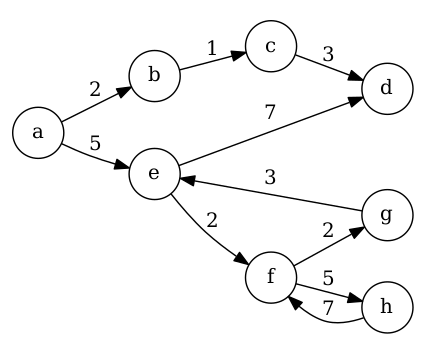
\includegraphics[width=\linewidth]{Immagini/example-waf-graph.png}
      \caption{Rappresentazione del grafo weighted.}
      \label{fig:waf-graph1}
    \end{figure}
    
    \label{exm:waf}
\end{exmp}

Ad esempi nel $WAF$ definito nell'esempio \ref{exm:waf}, l'insieme delle admissible extension è costituito da \{∅, \{a, c, f \}$, $\{a, f \}$, $\{a, c\}$, $\{a\}$, $\{g, h\}$, $\{h\}$, $\{a, c, g, h\}$, $\{a, c, h\}$, $\{a, g, h\}$, $\{a, h\}\}. L'insieme delle preferred extension è costituito da $\{\{a, c, f\}$, $\{a, c, g, h\}\}$. L'insieme delle complete extension è costituito da $\{\{a, c, g, h\}$, $\{a, c\}, \{a, c, f\}\}$. La grounded extension è costituita da $\{\{a, c\}\}$.

% ===================================================================
% ===================================================================
% ===================================================================
% ===================================================================

\subsection{Bipolar Weighted Argumetation Framework}

\begin{defn} \textbf{Bipolar Weighted Argumentation Framework}
Un Bipolar Weighted Argumentation Framework $(BWAF)$ è una tripla $\mathcal{A}$ è un insieme di argomenti, $\mathcal{R}$ è una relazione binaria e $w: \mathcal{R} \rightarrow [-1, 0)$ è una funzione che assegna un peso a ciascuna relazione. Dati due argomenti $a, b \in \mathcal{A}, a\mathcal{R}b \iff ⟨a,b ⟩\in \mathcal{R}$ indica che ha $a$ attacca $b$ se $-1 \leq (⟨a,b⟩) < 0$, altrimenti che $a$ supporta $b$ se $0 < w(⟨a,b⟩) \leq 1$.
\end{defn}

\bigskip
Un Bipolar Weighted Argumentation Framework $BWAF = ⟨\mathcal{A}, \mathcal{R}, w⟩$ può essere rappresentato come un grafo orientato e pesato $\mathcal{G} = ⟨\mathcal{V}, \mathcal{E}⟩$, dove l'insieme dei nodi $\mathcal{V}$ corrisponde all'insieme $\mathcal{A}$ e l'insieme degli archi $\mathcal{E}$ corrisponde all'insieme $\mathcal{R}$.

\bigskip
\begin{defn} \textbf{Relazione di attacco e di supporto}
Sia dato un Bipolar Weighted Argumentation Framework $BWAF = ⟨\mathcal{A}, \mathcal{R}, w⟩$. Definiamo la relazione binaria di attacco tra gli elementi di $\mathcal{A}$ come $\mathcal{R}_{def} = \{⟨a,b⟩ \in \mathcal{R} \ | \ -1 \leq w(⟨a, b⟩) < 0\} \subseteq \mathcal{R}$ e la relazione binaria di supporto tra gli elementi di $\mathcal{A}$ come $\mathcal{R}_{sup} = \{⟨a, b⟩ \in \mathcal{R} \ | \ 0 < w(⟨a, b⟩) \leq 1\} \subseteq \mathcal{R}$.
\end{defn}

\bigskip
\begin{exmp}
    Sia dato il $BWAF  = ⟨\mathcal{A}, \mathcal{R}, w⟩$, dove:
    \begin{center}
        $\mathcal{A} = ⟨a, b, c, d, e, f, g, h⟩$
        
        $\mathcal{R}_{def} = \{⟨c, d⟩, ⟨a, e⟩, ⟨e, f⟩, ⟨f, g⟩, ⟨g, e⟩, ⟨f, h⟩, ⟨h, f⟩\}$
        
        $\mathcal{R}_{sup} = \{⟨a, b⟩, ⟨b, c⟩, ⟨e, d⟩\}$
        
        $w(⟨a, b⟩) = 0.7, w(⟨b, c⟩) = 0.9, w(⟨c, d⟩) = -0.4, w(⟨a, e⟩) = -0.7, w(⟨e, d⟩) = 0.3, w(⟨e, f⟩) = -0.5, w(⟨f, g⟩) = -0.3, w(⟨g, e⟩) = -0.1, w(⟨f, h⟩) = -0.5, w(⟨h, f⟩) = -0.7$
    \end{center}
    
    \begin{figure}[h]
      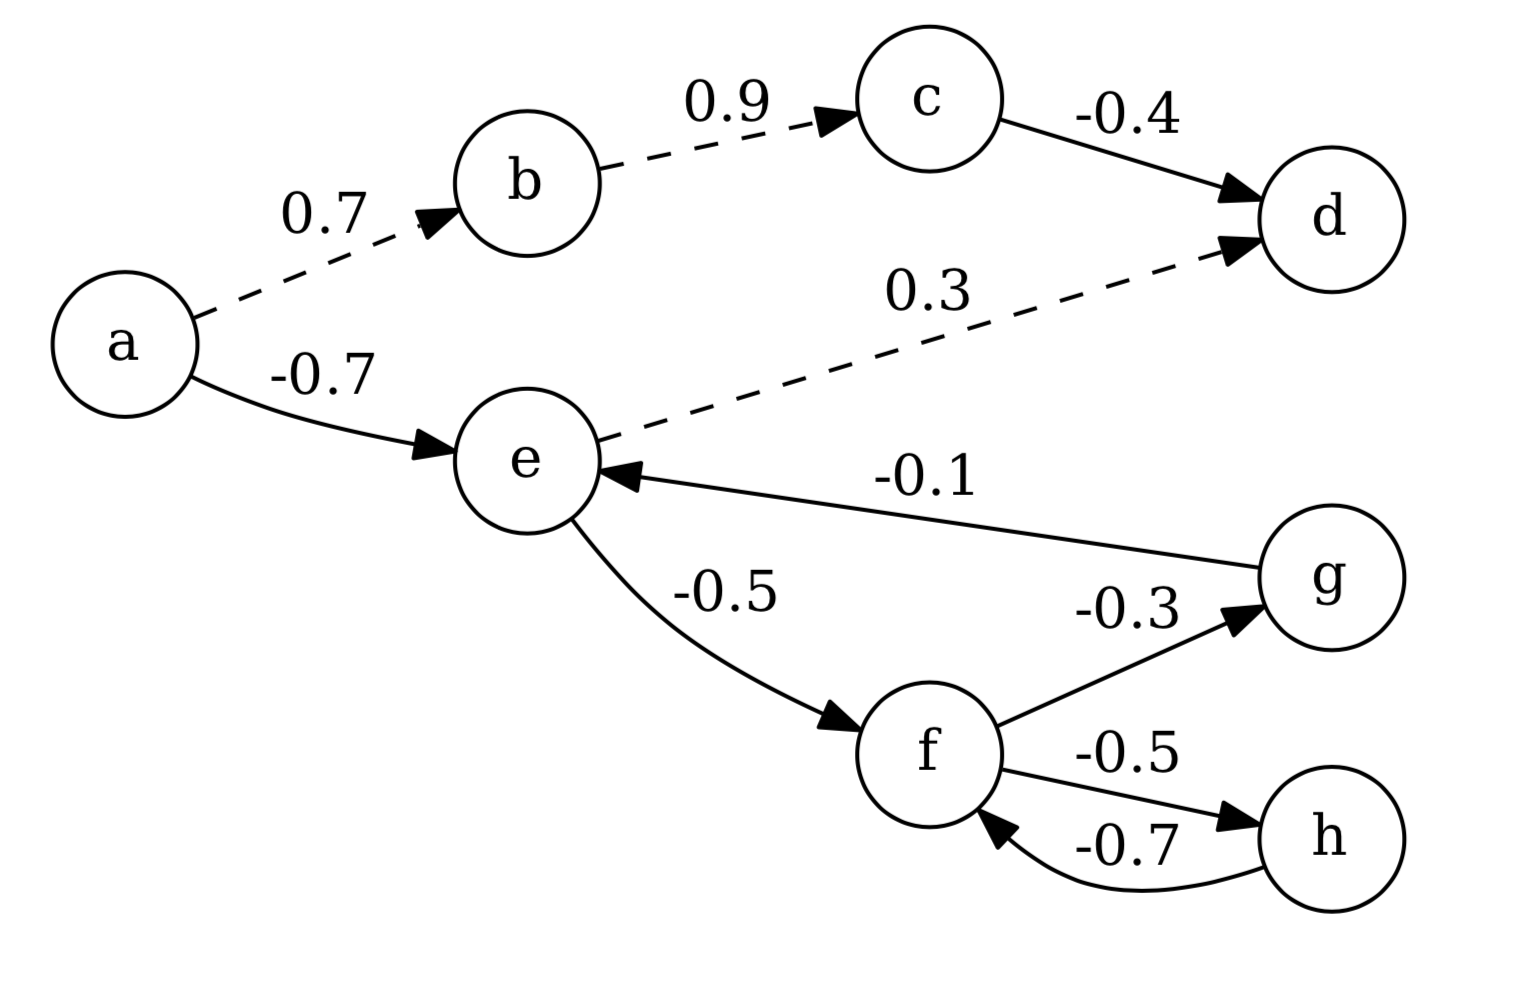
\includegraphics[width=\linewidth]{Immagini/example-bwaf-graph.png}
      \caption{Rappresentazione del BWAF.}
      \label{fig:bwaf-graph1}
    \end{figure}
    
    \label{exm:bwaf}
\end{exmp}

Alla luce delle definizioni di relazione di attacco $\mathcal{R}_{def}$ e di relazione di supporto $\mathcal{R}_{sup}$ riportate per il Bipolar Weighted Framework $BWAF = ⟨\mathcal{A}, \mathcal{R}, w⟩$, valgono le definizioni \ref{defn:adbaf}, \ref{defn:aibaf}, \ref{defn:asbaf}, \ref{defn:adibaf}, \ref{defn:sdibaf}, \ref{defn:dbaf} espresse per il $BAF = ⟨\mathcal{A}, \mathcal{R}_{def}, \mathcal{R}_{sup}⟩$.

\bigskip
\begin{defn} \textbf{Inconsistency budget}
Siano dati un bipolar argumentation $BWAF = ⟨\mathcal{A}, \mathcal{R}, w⟩$, una relazione $\mathcal{X} \subseteq \mathcal{R}$ e due inconsistency budget $\alpha \in \mathbb{R}_{<0}$, $\beta \in \mathbb{R}_{>0}$. Si definiscono le funzioni:

    \begin{center}
        
        $$wt(\mathcal{X}, w) = \sum_{⟨a, b⟩ \in \mathcal{X}}$$
        
        $sub_{def}(\mathcal{R},w,\alpha) = \{Y \ | \ Y \subseteq \mathcal{R} \land wt(\mathcal{R},w) \geq \alpha \}$
        
        $sub_{sup}(\mathcal{R},w,\beta) = \{Y \ | \ Y \subseteq \mathcal{R} \land wt(\mathcal{R},w) \leq \alpha \}$
        
        $\phi(\mathcal{A}, \mathcal{R}_{def}, \mathcal{R}_{sup}, \alpha, \beta) = 
        \{\mathcal{S} \subseteq \mathcal{A} \ | \ \exists \mathcal{R}_{\sigma} \in \{sub_{def}(\mathcal{R}_{def}, w, \alpha) \ \lor \ sub_{sup}(\mathcal{R}_{sup}, w, \beta) \} \land S \in \Theta (\mathcal{A}, \mathcal{R} \setminus \mathcal{R}_{\sigma}) \}$
        
    \end{center}
    
    dove $\Theta(\mathcal{A}, \mathcal{B})$ è un operatore che restituisce gli argomenti presenti in  $\mathcal{A}$ coinvolti nella relazione $\mathcal{B}$.

\end{defn}

A partire da $\phi(\mathcal{A}, \mathcal{R}_{def}, \mathcal{R}_{sup}, \alpha, \beta)$ si ottiene un sottoinsieme dell'insieme delle parti di $\mathcal{A}$ i cui elementi contengono solo argomenti che partecipano a relazioni con un peso inferiore ad $\alpha$ e superiore a $\beta$. Un insieme $\mathcal{S} \in \phi(\mathcal{A}, \mathcal{R}, \beta)$ può rientrare nelle estensioni definite per il framework di Dung al variare del parametro $\beta$. Per tale motivo, nei weighted argumentation framework, si parla di estensioni come la $\beta$-admissible, $\beta$-preferred e la $\beta$-grounded.
Ad esempio, dati gli inconsistency budget $\alpha = -0.3$ e $\beta = 0.3$, nel $BWAF$ definito nell'esempio \ref{exm:bwaf}, l'insieme delle $\alpha$-$\beta$-admissible extension è costituito da:  

\begin{center}
    $\{\varnothing,\{a,b,c,f,g\},\{a,c,f,g\},\{a,b,f,g\},\{a,f,g\},\{a,b,c,f\},\{a,c,f\},$ \\ 
    $\{a,b,f\},\{a,f\},\{a,b,c,g,h\},\{a,c,g,h\},\{a,b,g,h\},\{a,g,h\},\{a,b,c,h\},$ \\ 
    $\{a,c,h\},\{a,b,h\},\{a,h\},\{b,c,g,h\},\{b,g,h\},\{b,c,h\},\{b,h\},\{c,g,h\},$ \\ 
    $\{c,h\},\{g,h\},\{h\},\{a,b,c,g\},\{a,c,g\},\{a,b,g\},\{a,g\},\{a, b, c\}, \{a, c\}, \{a, b\},$ \\
    $\{a\}, \{b, c, g\}, \{b, g\},\{b, c\}, \{b\}, \{c, g\}, \{c\}, \{g\}\}$
\end{center}

Tale insieme è safe, per cui esso costituisce anche la $\alpha$-$\beta$-c-admissible extension del $BWAF$. L'insieme delle $\alpha$-$\beta$-c-admissible extension è, invece:

\begin{center}
    $\{\{g\},\{\},\{g,h\},\{h\},\{a,b,c,f,g\},\{a,b,c,f\},$ \\ 
    $\{a,b,c,g\},\{a,b,c\},\{a,b,c,g,h\},\{a,b,c,h\}$
\end{center}

Inoltre, l'insieme delle $\alpha$-$\beta$-d-preferred extension è costituito da:

\begin{center}
    $\{a,b,c,g,h\},\{a,b,c,f,g\}$
\end{center}

Tale insieme è safe, per cui esso costituisce anche la $\alpha$-$\beta$-s-preferred extension del $BWAF$. Inoltre, tale insieme soddisfa la proprietà di chiusura rispetto alla relazione di supporto e tale insieme difende se stesso, per cui è anche una $\alpha$-$\beta$-c-preferred extension.
Nella formalizzazione del $BWAF$ introdotta in questa sezione, si aggiunge un operatore in grado di valutare la forza di un attacco o di un supporto da un argomento verso un argomento non necessariamente in relazione diretta con esso. Si introduce, di seguito, la formalizzazione di tale operatore.

\bigskip
\begin{defn} \textbf{Argue}
Sia dato un Bipolar Weighted Argumentation Framework $BWAF = ⟨\mathcal{A}, \mathcal{R}, w⟩$. Definiamo la funzione$ path\_weight$ che calcola la forza di un cammino $v_1, ... , v_n$, dove $v_1 = a$, $v_n = b$ come il prodotto di $w(⟨v_{i-1},v_1⟩)$, $\forall i = 2,...,n$. Definiamo la funzione $node\_influence$ che calcola l'influenza di un argomento $a \in \mathcal{A}$ in base ai cicli a cui appartiene come $\prod_{a,...,a}$  $path\_weight(⟨a,...,a⟩)$, se $a$ appartiene ad almeno un ciclo, 1 altrimenti. Definiamo la funzione argue che calcola la forza di una relazione da $a \in A$ verso $b \in A$ nel seguente modo:

    \begin{center}
        $$argue(a,b) = \sum_{a,...,b} path_weight(⟨a,...,b⟩). \prod_{c \in ⟨a,...,b⟩} node\_influence(c)$$
    \end{center}

\end{defn}

In particolare, dati due argomenti $a$ e $b$, la definizione per la $argue(a,b)$ equivale a calcolare la somma delle forze di tutti i cammini da $a$ a $b$, ciascuna delle quali è ottenuta  come il prodotto dei pesi delle relazioni contenute nel cammino moltiplicato per il prodotto dell'influenza di ciascun argomento presente nel cammino. 

La motivazione legata a tale definizione è dovuta al fatto che tra due argomenti possono sussistere
cammini multipli costituiti da relazioni di attacco e di supporto, che hanno rispettivamente un
peso negativo e positivo. Inoltre, un argomento può essere coinvolto in più cicli, ciascuno dei
quali può contenere argomenti a loro volta coinvolti in altri cicli. 

Secondo la definizione data, la $argue(a,b)$ presenta un valore positivo se sussiste una difesa da $a$ verso $b$, negative sussiste un attacco tra di essi. Tale funzione rappresenta una misura complessiva della relazione che intercorre tra due argomenti nell'ambito di una intera discussione. Nell'esempio \ref{exm:bwaf}, la relazione da $a$ verso $d$ è calcolata nel seguente modo:

\begin{center}

    $path\_weight(⟨a,b,c,d⟩) = 0.7 \cdot 0.9 \cdot (-0.4) = -0.252$
    
    $path\_weight(⟨a,e,d⟩) = (-0.7) \cdot 0.3 = -0.21$
    
    $node\_influence(e) = path\_weight(⟨e,f,h,f,g,e⟩) =$ \\ 
    $= (-0.5) \cdot (-0.5) \cdot(-0.5) \cdot (-0.7) \cdot (-0.3) \cdot (-0.1) =$ \\
    $= -0.2508975$
    
\end{center}

Dall'esempio si evince che $a$ attacca $d$ con una forza pari a $a \approx -0.25$


\section{Argumetation Mining}
L'Argumentation Mining fornisce metodi per l'estrazione di argomenti da documenti testuali ed include molteplici sotto task come la identificazione degli argomenti e la scoperta della loro struttura. Molti ricercatori hanno già applicato l'Argumentation Mining in molti domini. Ad esempio in \cite{teufel1999annotation} si cerca di identificare argomenti nelle frasi di pubblicazioni scientifiche, in \cite{moens2007automatic} gli argomenti vengono estratti da documenti legali, in \cite{feng2011classifying} vengono analizzati articoli di giornale o in \cite{florou2013argument} nelle trascrizioni di casi giudiziari. The goal of argumentation mining, an evolving research field in computational linguistics, is to design methods capable of analyzing people’s argumentation.In general, the output of automatic argument analysis performed on the large scale in Web data can provide users with analyzed arguments to a given topic of interest, find the evidence for the given controversial standpoint, or help to reveal flaws in argumentation of others. As an emerging research area, argumentation mining still suffers from a lack of labeled corpora, which is crucial for designing, training, and evaluating the algorithms. Boltuzic  and Snajder (2014, page 50) point out that “unlike in debates or other more formal argumentation sources, the arguments provided by the users, if any, are less formal, ambiguous, vague, implicit, or often simply poorly worded.” Bentahar, Moulin, and Be langer (2010) propose a taxonomy of argumentation models that is horizontally divided into three categories: micro-level models, macro-level models, and rhetorical models. In this article, we deal with argumentation on the micro-level (also called argumen- tation as a product or monological models). Micro-level argumentation focuses on the structure of a single argument. By contrast, macro-level models (also called dialogical models) and rhetorical models highlight the process of argumentation in a dialogue (Bentahar, Moulin, and Be langer 2010, page 215). According to the classical Aristotelian theory (Aristo- tle and Kennedy [translator] 1991), argument can exist in three dimensions, which are logos, pathos, and ethos. The logos dimension represents a proof by reason, an attempt to persuade by establishing a logical argument. For example, syllogism be- longs to this argumentation dimension (Amossy 2009; Rapp and Wagner 2012). The pathos dimension makes use of appealing to emotions of the receiver and impacts its cognition (Micheli 2008). The ethos dimension of argument relies on the credibility of the arguer. This distinction will have practical impact later in Section 4.4, which deals with argumentation on the Web. Separation of Argumentative from Non-argumentative Text Units The first step of an argumentation mining pipeline typically focuses on the identification of argu- mentative text units before analyzing the compo- nents or the structure of arguments. This task is usually considered as a binary classification task that labels a given text unit as argumenta- tive or non-argumentative. One of the first ap- proaches was proposed by (Moens et al., 2007). They focus on the identification of argumentative text units in newspaper editorials and legal doc- uments included in the Araucaria corpus (Reed et al., 2008). The annotation scheme utilized in Araucaria is based on a domain-independent ar- gumentation theory proposed by Walton (1996). A similar approach is reported by Florou et al. (2013). In their experiments, they classify text segments crawled with a focused crawler as either containing an argument or not. They focus on the identification of arguments in the policy model- ing domain for facilitating decision making. For that purpose, they utilize several discourse mark- ers and features extracted from the tense and mood of verbs. Although the separation of argumentative from non-argumentative text units is an important step in argumentation mining, it merely enables the de- tection of text units relevant for argumentation and does not reveal the argumentative role of argument components. 3.2 Classification of Argument Components The classification of argument components aims at identifying the argumentative role (e.g. claims and premises) of argument components. One of the first approaches to identify argument components is Argumentative Zoning proposed by (Teufel, 1999). Each sentence is classified as one of seven rhetorical roles including e.g. claim, re- sult or purpose using structural, lexical and syn- tactic features. The underlying assumption of this work is that argument components extracted from a scientific article provide a good summary of its content. Rooney et al. (2012) also focus on the identification of argument components but in con- trast to the work of Teufel (1999) their scheme is not tailored to a particular genre. In their exper- iments, they identify claims, premises and non- argumentative text units in the Araucaria corpus. Feng and Hirst (2011) also use the Araucaria cor- pus for their experiments, but focus on the identi- fication of argumentation schemes (Walton, 1996) which are templates for arguments (e.g. argument from example or argument from position to know). Since their approach is based on features extracted from mutual information of claims and premises, it requires that the argument components are re- liably identified in advance. Mochales-Palau and Moens (2009) report several experiments for clas- sifying argument components. They solely focus on the legal domain and in particular on legal court cases from the European Court of Human Rights (ECHR). They consider the classification of argu- ment components as two consecutive steps. They utilize a maximum entropy model for identifying argumentative text units before identifying the ar- gumentative role (claim and premise) of the identi- fied components using a Support Vector Machine. 3.3 Identification of Argumentation Structures Currently, there are only few approaches aiming at the identification of argumentation structures. For instance, the approach proposed by Mochales- Palau and Moens (2011) relies on a manually created context-free grammar (CFG) and on the presence of discourse markers for identifying a tree-like structure between argument components. However, the approach relies on the presence of discourse markers and exploits manually created rules. Therefore, it does not accommodate ill- formatted arguments (Wyner et al., 2010) and is not capable of identifying implicit argumentation structures which are common in argumentative discourse. Indeed, Marcu and Echihabi (2002) found that only 26\% of the evidence relations in the RST Discourse Treebank (Carlson et al., 2001) include discourse markers. Another approach was presented by Cabrio and Villata (2012). They identify relations between ar- guments of an online debate platform for identify- ing accepted arguments and to support the interac- tions in online debates. In contrast to the work of Mochales-Palau and Moens (2011), this approach aims at identifying relations between arguments (macro-level) and not between argument compo- nents (micro-level).